\subsection{Group source reconstruction}

\begin{figure}
\centering
\begin{minipage}{0.35\linewidth}
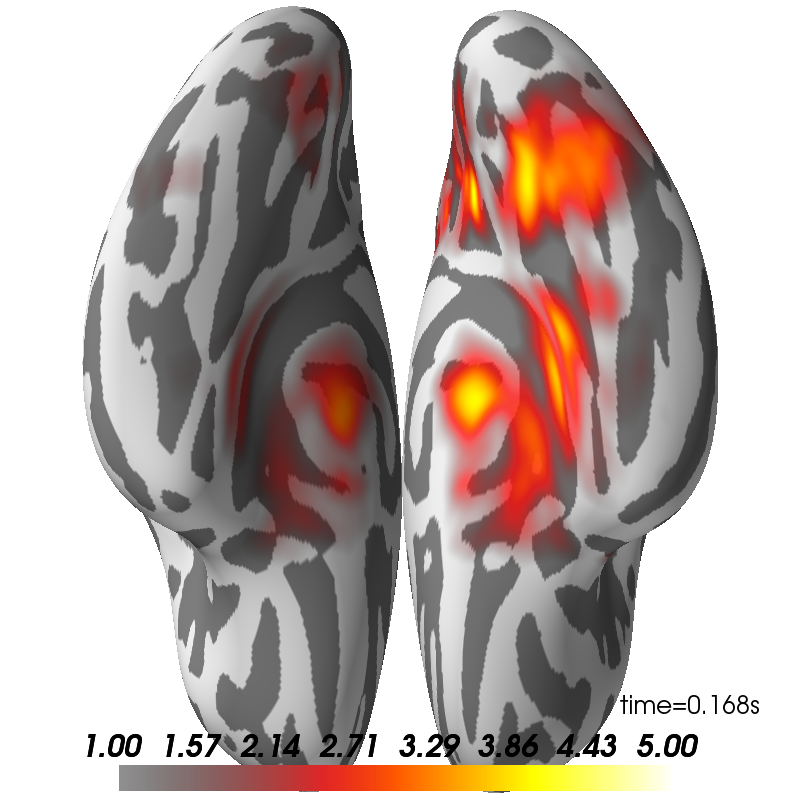
\includegraphics[width=\linewidth]{figures/dspm-ave_highpass-NoneHz.png}
\end{minipage}
\begin{minipage}{0.35\linewidth}
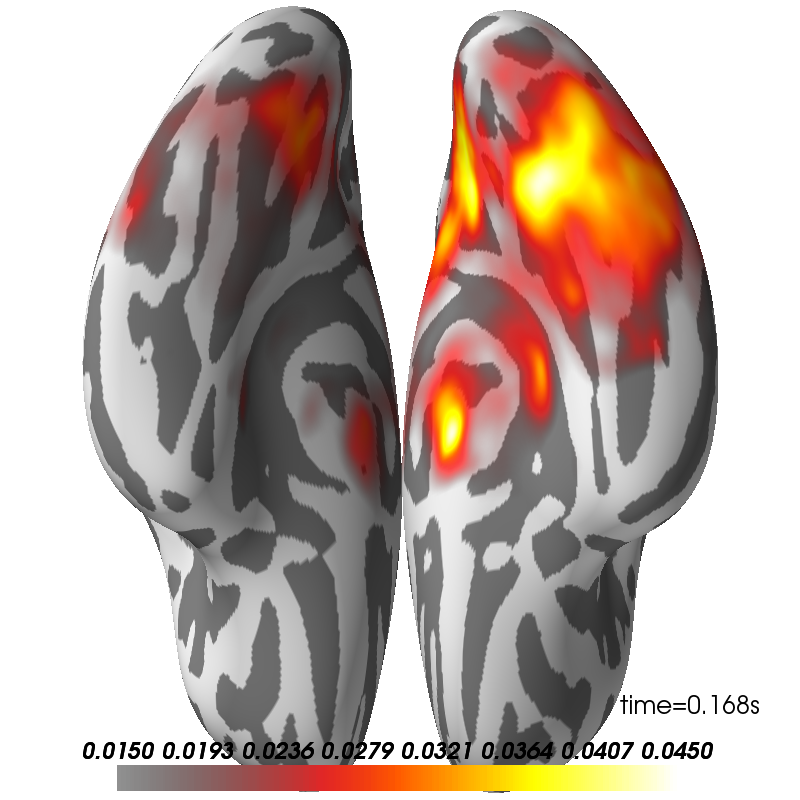
\includegraphics[width=\linewidth]{figures/lcmv-ave_highpass-NoneHz.png}
\end{minipage}
\caption[Group average on source reconstruction with dSPM and LCMV.]{Group average on source reconstruction with dSPM (left) and LCMV (right). Here, we have the ventral view of an inflated surface with the anterior-posterior line going from the bottom to top of the image. Right hemisphere is on the right side.}
\label{fig:fig_stc}
\end{figure}

To analyze data at the group level, some form of data normalization is necessary, whereby data from all subjects is transformed to a common space in a manner that helps compensate for inter-subject differences. This procedure, called \emph{morphing} by the MNE software, exploits the FreeSurfer spherical coordinate system defined for each hemisphere~\citep{dale-fischl-etal:99,fischl-serena-etal:99}. In our analysis, the data are morphed to the standard FreeSurfer average subject named \code{fsaverage}. The morphing procedure is performed in three steps. First, the subsampled data defined on the high resolution surface are spread to neighboring vertices using an isotropic diffusion process. Next, registration is used to interpolate the data on the average surface. And finally, the data defined on the average surface is subsampled to yield the same number of source locations in all subjects (here, 10242 locations per hemisphere). Once the morphing is complete, the data is simply averaged.

What is presented in Figure~\ref{fig:fig_stc} is the group average of the dSPM and LCMV beamformer solutions on contrast between faces and scrambled
at 170\,ms post-stimulus.

Looking at these results, one can observe that both methods highlight a peak of activation on the right ventral visual cortex known to be involved in face processing~\citep{grill2017functional,grill2004fusiform,wakeman2015multi}. The dSPM peak seems however to be slightly more anterior.

\subsection{Source-space statistics}

\begin{figure}
\centering
\begin{minipage}{0.4\linewidth}
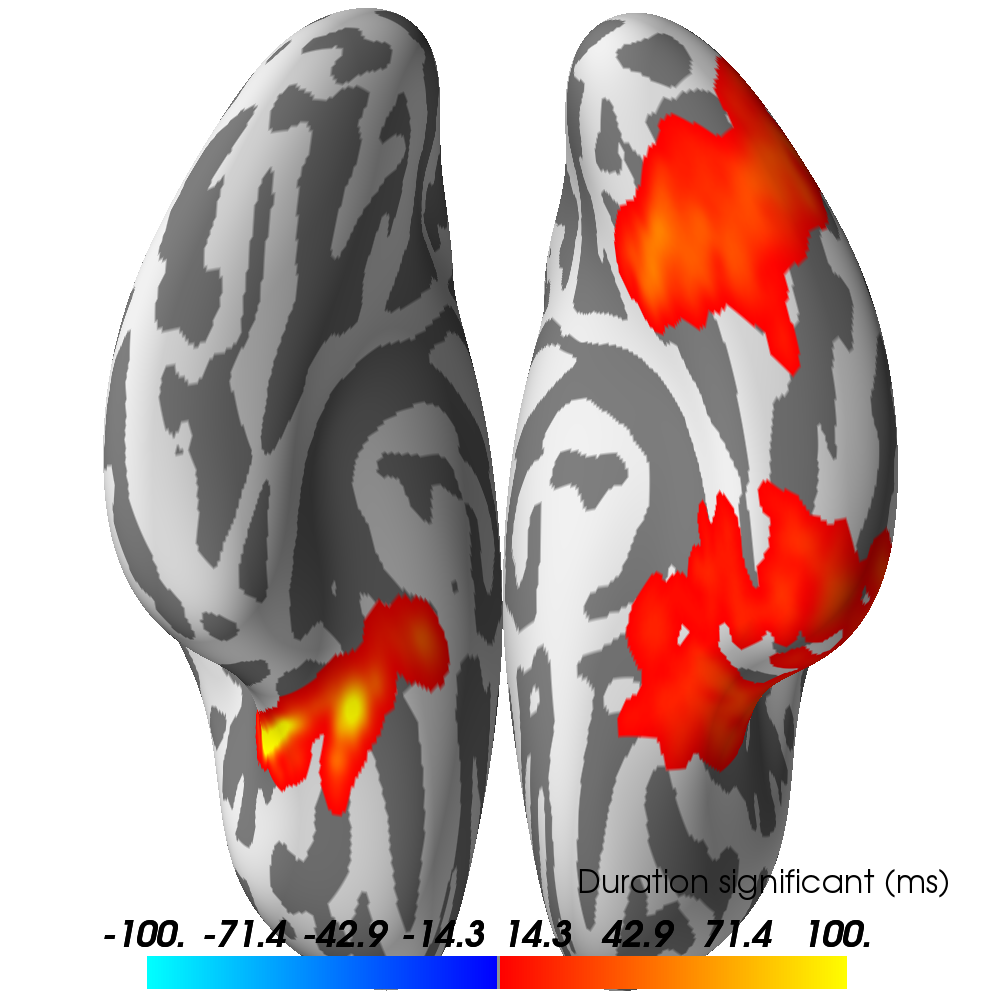
\includegraphics[width=\linewidth]{figures/source_stats_highpass-NoneHz.png}
\end{minipage}
\caption[Spatio-temporal source space clusters obtained by nonparametric permutation test.]{Spatio-temporal source space clusters obtained by nonparametric permutation test that allowed rejection of the null hypothesis that the distribution of data for the "faces" condition was the same as that of "scrambled". The clusters here are collapsed across time such that vertex colors indicate the duration that each vertex was included in its cluster (each cluster here occurring with FWER corrected $p < 0.05$). Hot colors indicate durations for vertices in clusters where response for faces $>$ scrambled (cool colors would be used for scrambled $>$ faces, but no such clusters were found).}
\label{fig:fig_source_stats}
\end{figure}

Just as we did for the sensor time courses, we can subject the source time courses (here for dSPM only) to a cluster-based permutation test. The null hypothesis is again that there is no significant difference between the data distributions (here measured using cluster size) for faces versus scrambled (paired). Under each permutation, we do a paired t-test across subjects for the difference between the (absolute value of the) faces and scrambled values for each source space vertex and time point. These are clustered, and maximal cluster size for each permutation is selected to form the null distribution. Cluster sizes from the actual data are compared to this null; in this case we find three clusters that lead us to reject the null with $p < 0.05$ (see Figure~\ref{fig:fig_source_stats}).
 
 \emph{Alternatives} When strong hypotheses exist with regard to spatial, temporal and spectral regions of interest, it may be preferable to test the experimental hypotheses on fewer well-chosen signals. In the context of a group analysis, a linear multilevel modeling approach may provide an interesting option for obtaining joint inference at the single subject and group level~\cite{gelman2006multilevel,baayen2008mixed}.
 
% \begin{figure}[htbp]
%     \centering
%         \includegraphics[width=\linewidth]{morphing.jpg}
%     \caption{Current estimates obtained from an individual subject can be remapped (morphed),
%     {\em i.e.}, normalized, to another cortical surface, such as that of the FreeSurfer average brain ``\emph{fsaverage}''
%     shown here. The normalization is done separably for both hemispheres using a non-linear registration
%     procedure defined on the sphere~\citep{dale-fischl-etal:99,fischl-serena-etal:99}.
%     Here, the N100m auditory evoked response is localized usin g dSPM and then mapped to
%     ``fsaverage''. \REV{Images were produced with {\em PySurfer}.}}
%     \label{fig:morphing}
% \end{figure}
